\documentclass[a4paper,10pt]{article}
\usepackage[utf8]{inputenc}
\usepackage[slovak]{babel}
\usepackage{amsmath}
\usepackage{graphicx}
\usepackage{hyperref}
\hypersetup{
    colorlinks=false,
}

\usepackage[left=3.0cm,
			right=3.0cm,
			top=1.5cm,
			bottom=1.5cm,
			]{geometry}
\begin{document}


\title{Korekčné členy}

\author{Martin Dodek}
\pagestyle{plain}
\maketitle


Riadený systém nech má tvar prenosovej funkcie:
\begin{equation}
\label{eq:riadený systém}
F(s)=\frac{y(s)}{u(s)}=\frac{B(s)}{A(s)}
\end{equation}

Všeobecná prenosová funkcia korekčného člena má tvar:
\begin{equation}
 \label{eq:prenosová funkcia korekčného člena}
 C(s)=\frac{u(s)}{e(s)}=\frac{aTs+1}{Ts+1}
\end{equation}
Kde $T$ je časová konštanta ovplyvňujúca pracovnú (``strednú'') frekvenciu $\omega_m$, $a$ je parameter určujúci výsledný dynamický charakter korekčného člena.

Podľa hodnoty parametra $a$ rozlišujeme:
\begin{itemize}
	\item Korekčný člen s fázovým predstihom (Lead) $a>1$
	\item Korekčný člen s fázovým zaostávaním (Lag) $a<1$
\end{itemize}

\begin{figure}[ht]
\centering
\includegraphics[width=0.75\textwidth]{blokova_schema}
\caption{Bloková schéma URO s korekčným členom}
\end{figure}


\section{Frekvenčná prenosová funkcia}
Substitúciou $s=j\omega$ do prenosovej funkcie \eqref{eq:prenosová funkcia korekčného člena} získame frekvenčnú prenosovú funkciu korekčného člena, ktorá nadobudne tvar (bez odvodenia)\footnote{Odvodenie si každý spraví sám}:
\begin{equation}
\label{eq:frekvenčná prenosová funkcia korekčného člena}
 C(j\omega)=\frac{aTj\omega+1}{Tj\omega+1}=\frac{aT^2\omega^2+1}{T^2\omega^2+1}+\frac{T\omega(a-1)}{T^2\omega^2+1}j
\end{equation}

Pre fázový posun bude potom platiť:
\begin{equation}
\label{eq:frekvenčná prenosová funkcia fáza}
 \arg(C(j\omega))=\arctan{\frac{T\omega(a-1)}{aT^2\omega^2+1}}
\end{equation}

\pagebreak

\section{Návrh parametra $T$} 
Pri návrhu uvažujeme posunutie frekvencie pôvodného amplitúdového priesečníka na novú hodnotu $\omega_m$.
Hľadáme frekvenciu nového amplitúdového priesečníka, pri ktorej je nekorigovaná amplitúda rovná:
\begin{equation}
 -10\log(a)
\end{equation}

Táto frekvencia je zviazaná s parametrami korekčného člena a s jeho pracovnou frekvenciou $\omega_m$:
\begin{equation}
\label{eq:omega_m}
\omega_m=\frac{1}{T\sqrt{a}}
\end{equation}

Potom pre parameter $T$ bude platiť:
\begin{equation}
\label{eq:T}
 T=\frac{1}{\omega_m\sqrt{a}}
\end{equation}

Tu predpokladáme, že parameter $a$ už bol navrhnutý. To znamená, že najprv začíname návrhom $a$ a pokračujeme výpočtom $T$.

\section{Návrh parametra $a$} 
Fázový posun pri frekvencii $\omega_m$ je možné určiť na základe rovnice \eqref{eq:frekvenčná prenosová funkcia fáza} a rovnice \eqref{eq:omega_m}.
\begin{equation}
 \phi_m=\arg(C(\omega_m))=\arctan{\frac{a-1}{2\sqrt{a}}}
\end{equation}

\begin{equation}
 \sin(\phi_m)=\frac{\tan(\phi_m)}{\sqrt{\tan^2(\phi_m)+1}}
\end{equation}

\begin{equation}
 \sin(\phi_m)=\frac{\frac{a-1}{2\sqrt{a}}}{\left({\frac{a-1}{2\sqrt{a}}}\right)^2+1}=\frac{a-1}{a+1}
\end{equation}

Po úprave získame vzťah pre parameter $a$
\begin{equation}
\label{eq:a}
 a=\frac{1+\sin(\phi_m)}{1-\sin(\phi_m)}
\end{equation}

Potrebné fázové prevýšenie korekčného člena $\phi_m$ určíme ako rozdiel požadovanej fázovej bezpečnosti $\phi_z$ a fázovej rezervy riadeného systému $\phi_0$ (tú získame grafickým odčítaním z Bodeho charakteristiky):
\begin{equation}
\label{eq:phi_m}
\phi_m=\phi_z-\phi_0
\end{equation}

\pagebreak

\section{Návrh zosilnenia $K$} 
Požadujme trvalú regulačnú odchýlku riadenia:
\begin{equation}
\epsilon=e(\infty)
\end{equation}

Zvyčajne v intervale $\left<0.001 \ldots 0.1 \right>$.

Statické zosilnenie riadeného systému \eqref{eq:riadený systém} vieme určiť ako:
\begin{equation}
\label{eq:g_F}
g_F=\frac{b_0}{a_0}
\end{equation}

Statické zosilnenie uzatvoreného regulačného obvodu bude:
\begin{equation}
 \frac{K g_F}{K g_F+1}
\end{equation}

Predpísaním trvalej regulačnej ochýlky požadujeme rovnosť:
\begin{equation}
1-\epsilon=\frac{K g_F}{K g_F+1}
\end{equation} 

Potom pre parameter zosilnenia $K$ korekčného člena musí platiť:
\begin{equation}
\label{eq:K}
K=\frac{1-\epsilon}{\epsilon g_F}
\end{equation}

\begin{figure}[ht]
\centering
\includegraphics[width=0.9\textwidth]{prechodova_charakteristika}
\caption{Prechodová charakteristika URO}
\end{figure}

\pagebreak

\section{Bodeho charakteristika Lead a Lag korekčného člena}
Lead korekčný člen má charakter hornopriepustného filtra. Pri frekvencii $\omega_m$ dochádza ku kladnému a zároveň najväčšiemu fázovému posunu.
\begin{figure}[ht]
\centering
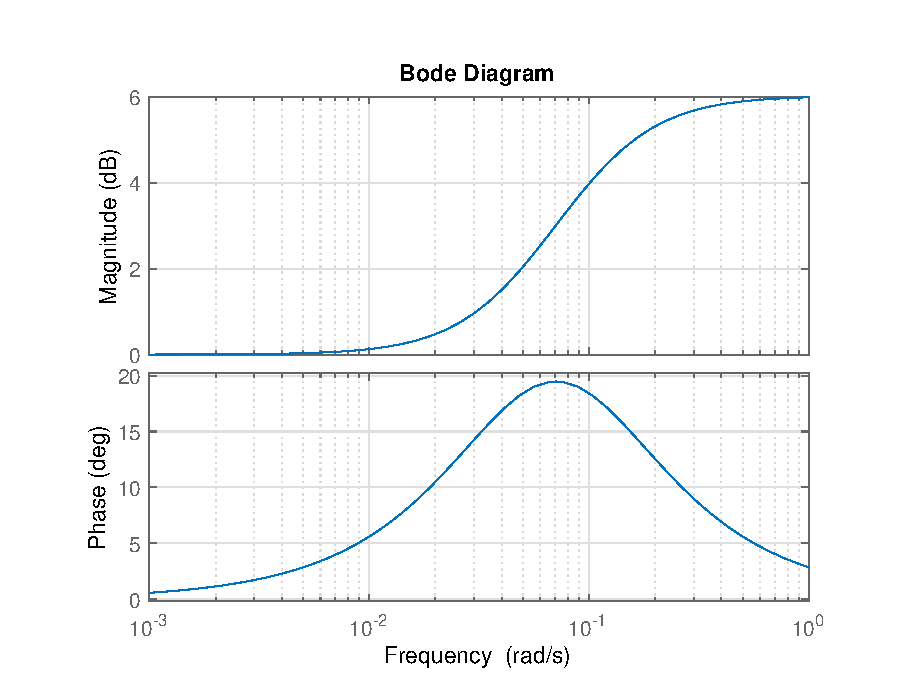
\includegraphics[width=0.77\textwidth]{LeadBode}
\caption{Frekvenčná charakteristika Lead korekčného člena}
\end{figure}

Lag korekčný člen má charakter dolnopriepustného filtra. Pri frekvencii $\omega_m$ dochádza k zápornému a zároveň najväčšiemu fázovému posunu.
\begin{figure}[ht]
\centering
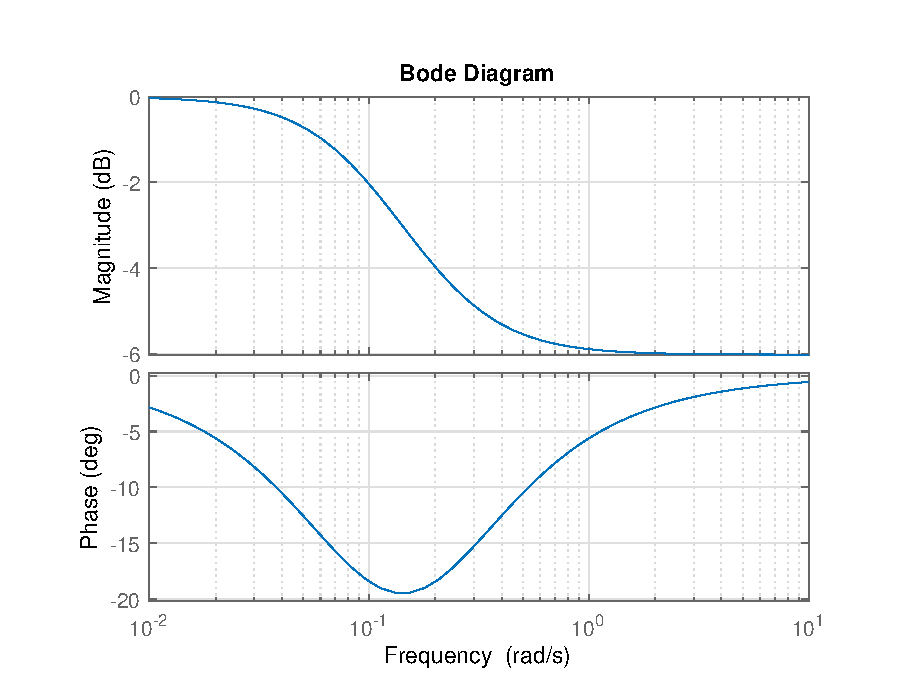
\includegraphics[width=0.77\textwidth]{LagBode}
\caption{Frekvenčná charakteristika Lag korekčného člena}
\end{figure}

\pagebreak

\section{Príklad}

Majme riadený systém v tvare prenosovej funkcie:
\begin{equation}
 F(s)=\frac{100}{(s+1)(s+2)(s+3)}
\end{equation}
Navrhnite Lead korekčný člen s požadovanou fázovou bezpečnosťou $\phi_z=45^\circ$ a s trvalou regulačnou odchýlkou $\epsilon=0.05$.

Určíme statické zosilnenie systému na základe rovnice \eqref{eq:g_F} ako:
\begin{equation}
   g_F=\frac{50}{3}
\end{equation}

Na základe rovnice \eqref{eq:K} vypočítame zosilnenie $K$
\begin{equation}
 K=\frac{1-\epsilon}{\epsilon g_F}=1.1400
\end{equation}

Z frekvenčnej charakteristiky riadeného systému určíme fázovú rezervu:

\begin{equation}
 \phi_0=-15^\circ
\end{equation}

Použitím rovnice \eqref{eq:phi_m} vypočítame potrebné fázové prevýšenie korekčného člena:

\begin{equation}
\phi_m=\phi_z-\phi_0=60^\circ
\end{equation}

Z fázového prevýšenia teraz vieme určiť parameter $a$, ako je definované v rovnici \eqref{eq:a}.
\begin{equation}
 a=\frac{1+\sin(\phi_m)}{1-\sin(\phi_m)}=13.9282
\end{equation} 

Následne je potrebné odhadnúť frekvenciu nového amplitúdového priesečníka.
Na frekvenčnej charakteristike riadeného systému nájdeme frekvenciu, pri ktorej je apmlitúda rovná:
 
\begin{equation}
 -10\log(a)=-11.4390\: dB
\end{equation}
A teda:

\begin{equation}
 \omega_m=6.85
\end{equation}

\begin{figure}[ht]
\centering
\includegraphics[width=0.9\textwidth]{SystemBode}
\caption{Frekvenčná charakteristika riadeného systému}
\end{figure}

\pagebreak

Teraz už vieme navrhnúť aj parameter $T$, tak ako je definované v rovnici \eqref{eq:T}.

\begin{equation}
 T=\frac{1}{\omega_m\sqrt{a}}=0.0391
\end{equation}  

Výsledná prenosová funkcia korekčného člena \eqref{eq:prenosová funkcia korekčného člena} potom bude:

\begin{equation}
 C(s)=\frac{aTs+1}{Ts+1}=1.14\:\frac{0.5448s+1}{0.03912s+1}
\end{equation}

\begin{figure}[ht]
\centering
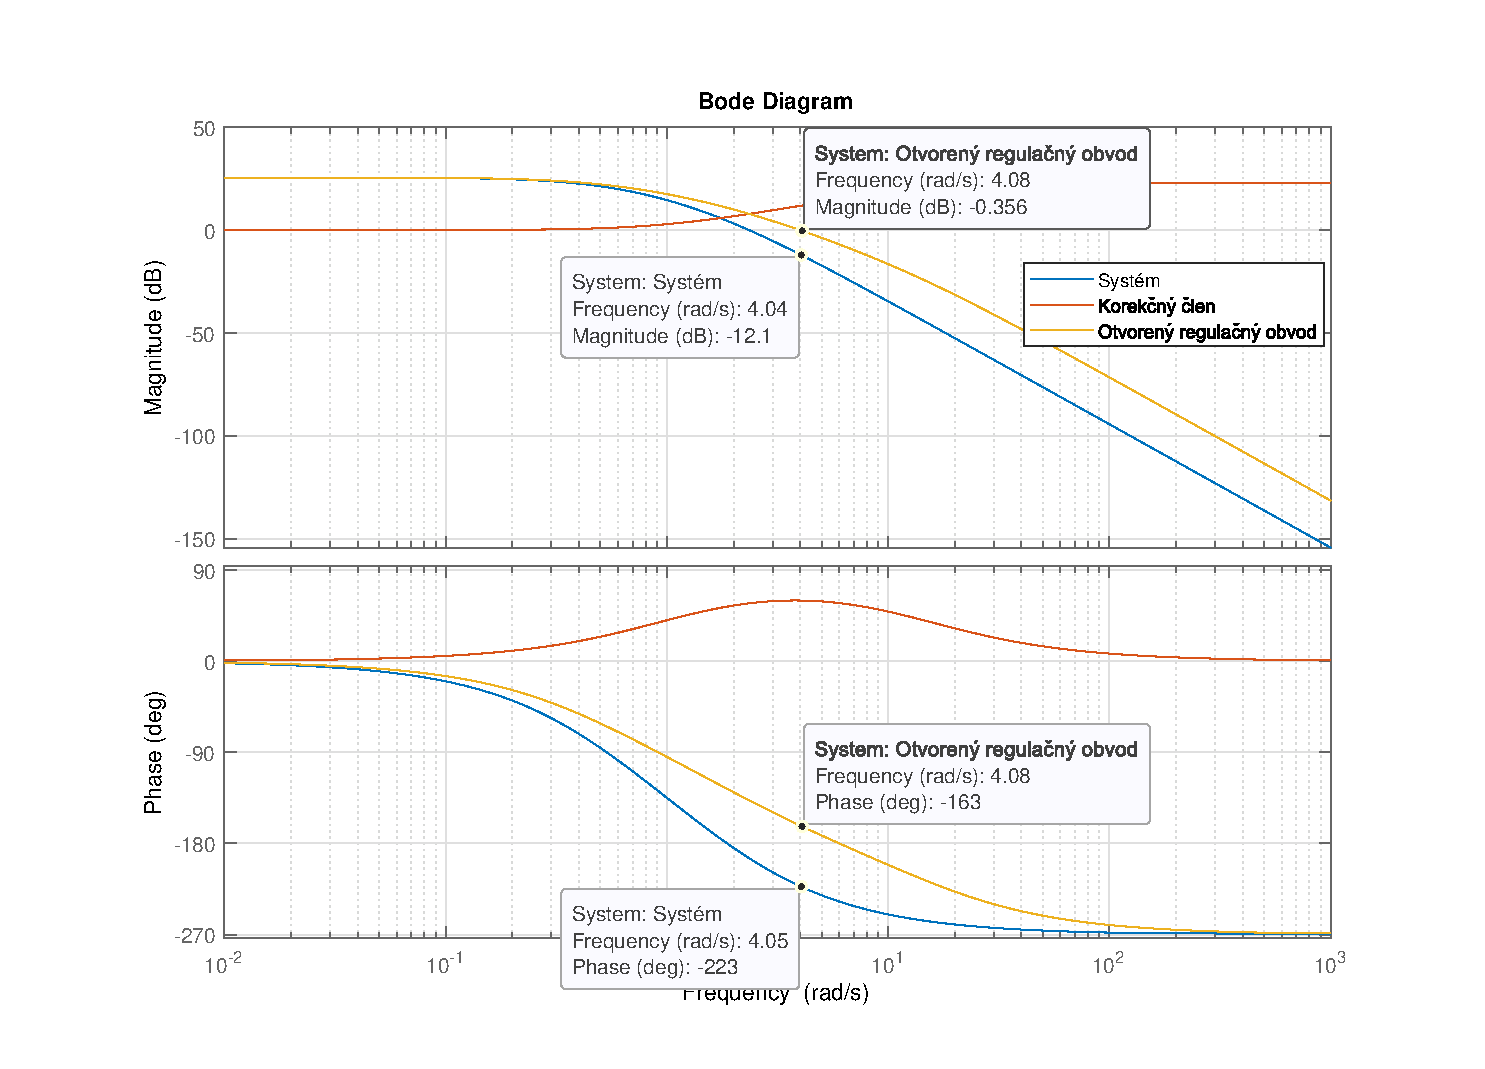
\includegraphics[width=1.0\textwidth]{OROBode}
\caption{Frekvenčná charakteristika otvoreného regulačného obvodu, korekčného člena a riadeného systému}
\end{figure}

\end{document}